\documentclass[a4paper]{article}

\usepackage[T1]{fontenc}
\usepackage[italian]{babel}
\usepackage[latin1]{inputenc}
\usepackage{graphicx}
\usepackage{float}
\usepackage[margin=2 cm]{geometry}
\usepackage{multirow}
\usepackage{multicol}
\usepackage{textcomp}
\usepackage{caption}

\author{Alberto Bordin, Giulio Cappelli}
\title{Laser a diodo}
\date{7-8 novembre 2017}

\begin{document}
	\maketitle
	
\begin{abstract}
	Misura della corrente di soglia di un diodo laser per varie temperature di operazione. \\
	Misura della divergenza del fascio. \\
	Misura della dipendenza della lunghezza d'onda dalla temperatura. \\
\end{abstract}

\section{To do}
\begin{itemize}
\item Foto apparato
\item Trovare informazioni fotodiodo
\end{itemize}

\begin{multicols}{2}

\section{Teoria}

\section{Apparato sperimentale}
Come si vede in Figura per poter effettuare le varie misure abbiamo a disposizione:
\begin{itemize}
\item Un laser a diodo modello \texttt{HL7812G} prodotto dalla \texttt{Hitachi}.
\item Un circuito di controllo in corrente del laser.
\item Una cella peltier, controllata in corrente, che utilizziamo per variare la temperatura del laser.
\item Un sensore ti temperatura \texttt{DIGIMASTER DM102}
\item Un analizzatore di spettro \texttt{USB4000} della \texttt{Ocean Optics}.
\item Una fibra ottica utilizzata per portare il segnale del laser al monocromatore.
\item Un piccolo ventilatore montato in modo tale da evitare la formazione di gocce d'acqua all'interno del laser durante i processi di riscaldamento e/o raffreddamento del laser.
\item Una lente utilizzata per focalizzare il laser nella misura della caratteristica P-I.
\item Un supporto per il laser montato su un goniometro con una precisione di 0.5�.
\item Un fotodiodo \texttt{PD300} della \texttt{Ophir}.
\item Un altro fotodiodo di cui non sappiamo niente.
\item Un power meter \texttt{NOVA} della \texttt{Ophir}.
\item Un rilevatore IR per poter osservare il fascio laser ed allinearlo.
\end{itemize}

\subsection{Laser a diodo}
Il laser a diodo a nostra disposizione � il modello \texttt{HL7812G} della \texttt{Hitachi} ed � una giunzione di GaAlAs. 

Sul datasheet sono riportate le seguenti caratteristiche:
\begin{table}[H]
\centering
\begin{tabular}{cccc}
	 & Min & Tipico & Max \\
	\hline
	I$_{th}$ [mA] & \textthreequartersemdash & 50 & 90 \\ 
	$\lambda_{p}$ [nm] & 770 & 785 & 795 \\
	$\theta_{//}$ [deg] & 7 & 11 & 18 \\
	$\theta_{\perp}$ [deg] & 20 & 30 & 40 \\
	\hline

\end{tabular}
\caption{Caratteristiche laser a diodo \texttt{HL7812G} misurate a T=25�C}
\end{table}
dove I$_{th}$ � la corrente di soglia oltre la quale si � in regime laser, $\lambda_{p}$ � la lunghezza d'onda della luce in uscita dal laser e $\theta_{//}$ e $\theta_{\perp}$ sono gli angoli di emissione del laser rispetto agli assi della giunzione e sono calcolati misurando l'intensit� ad una distanza di 10 cm dal diodo.

Sono inoltre presenti sul datasheet i seguenti grafici:
\begin{figure}[H]
\centering
\begin{minipage}[c]{0.24\textwidth}
\centering
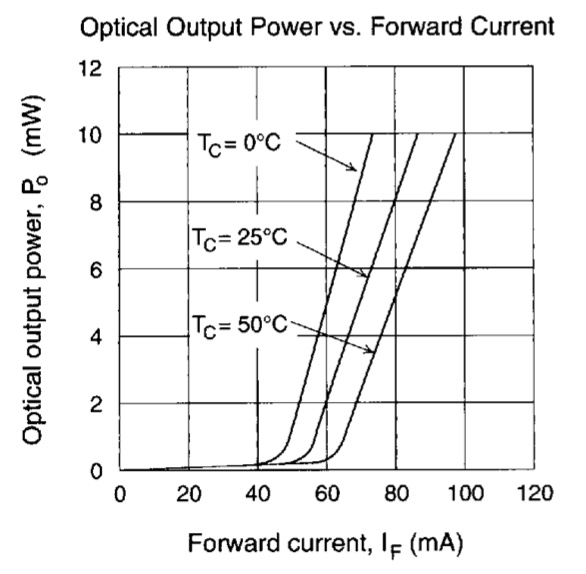
\includegraphics[width=\textwidth]{I_soglia}
\caption{}
\label{fig:I_soglia}
\end{minipage}
\begin{minipage}[c]{0.24\textwidth}
\centering
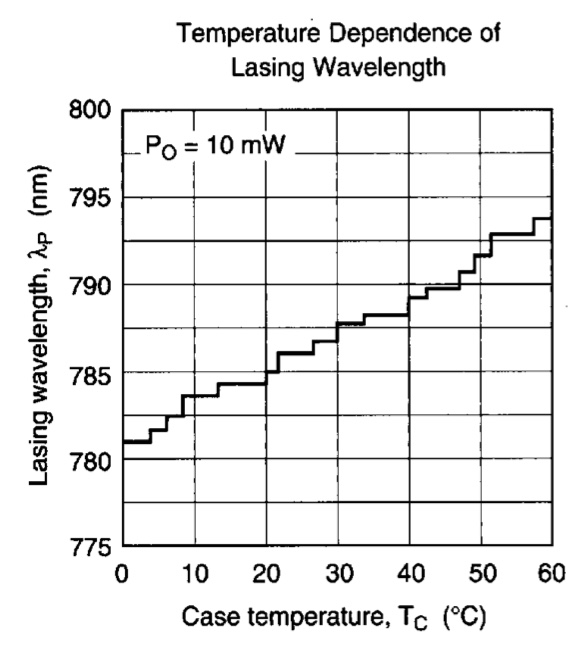
\includegraphics[width=\textwidth]{LambdavsT}
\caption{}
\label{fig:LambdavsT}
\end{minipage}
\end{figure}

\begin{figure}[H]
\centering
\includegraphics[width=0.4\textwidth]{IvsAng}
\caption{}
\label{fig:IvsAng}
\end{figure}

che mostrano le caratteristiche principali di dispositivi di questo tipo come la dipendenza della corrente di soglia dalla temperatura, l'astigmatismo e la dipendenza della lunghezza d'onda dalla temperatura.

\subsection{Monocromatore}
L'analizzatore di spettro � costituito da un monocromatore, ovvero un apparato in grado di sfruttare un reticolo di diffrazione (costituito da $\sim$1000 specchi $\forall$ mm) in riflessione per separare angolarmente le lunghezze d'onda della luce incidente. 
Prendendo come riferimento la Figura \ref{fig:monocromatore} si nota la presenza di due specchi (4 e 6) che servono, rispettivamente, a collimare il fascio sul reticolo di diffrazione e a focalizzare il primo ordine dello spettro sull'array di fotodiodi (8) che permettono di rilevare l'intensit� delle varie lunghezze d'onda che compongono la luce incidente.

Quello a nostra disposizione � un \texttt{USB4000} della \texttt{Ocean Optics} mostrato in Figura \ref{fig:monocromatore}, a cui la luce laser viene portata tramite una fibra ottica.

\begin{figure}[H]
\centering
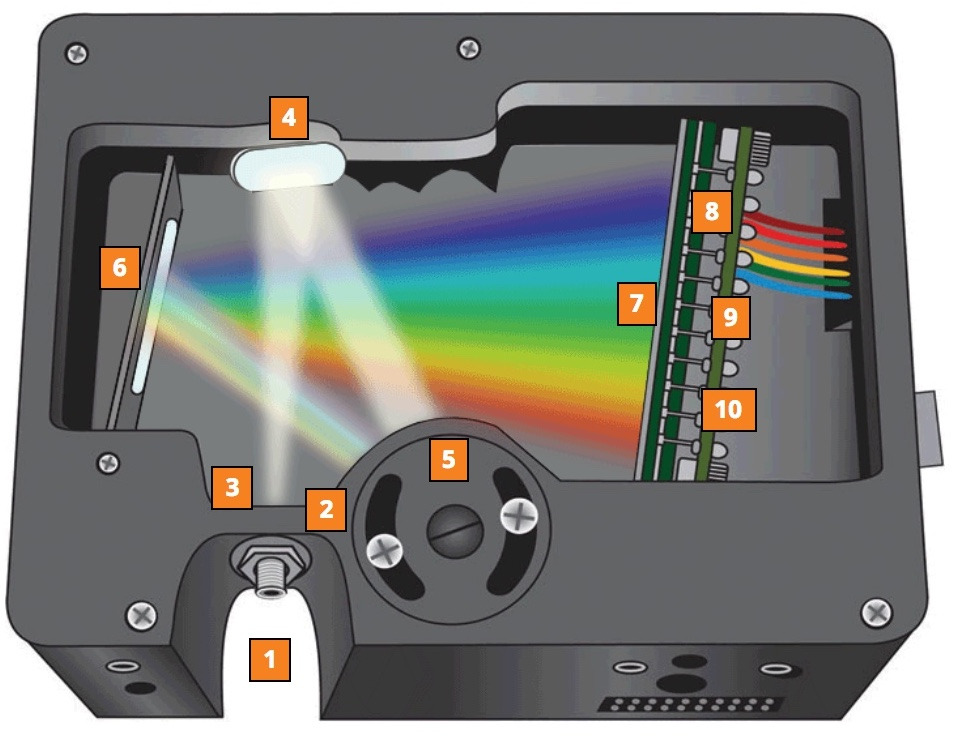
\includegraphics[width=0.4\textwidth]{monocromatore}
\caption{}
\label{fig:monocromatore}
\end{figure}

\section{Caratteristica P-I}
Analizziamo la dipendenza della corrente di soglia del diodo laser dalla temperatura misurando la caratteristica P-I in tre diverse condizioni: T=12, 25, 45 �C.

\subsection{Presa dati}
Abbiamo misurato la potenza fornita dal diodo laser in funzione della corrente di alimentazione mantenendo la temperatura del diodo costante attraverso l'utilizzo della cella peltier.

Il fascio � stato focalizzato sul fotodiodo attraverso una lente e per ogni valore della corrente abbiamo registrato il corrispondente valore della potenza leggendolo sul power meter NOVA RS232.

Abbiamo effettuato questa misura per tre valori diversi della temperatura del laser a diodo; tutte le misure effettuate sono riportate nelle rispettive tabelle in appendice.

Per ogni valore della temperatura � stato impostato sul power meter il valore previsto della lunghezza d'onda del laser a diodo come riportato sul datasheet (Figura \ref{fig:LambdavsT}).

\begin{table}[H]
\centering
\begin{tabular}{c|c|c|c}
	\hline
	T [�C] & 12 & 25 & 43 \\ 
	$\lambda$ [nm] & 784 & 786 & 790 \\
	\hline

\end{tabular}
\caption{}
\end{table}


\subsection{Analisi dati}

\section{Divergenza del fascio}

In questa seconda sezione calcoliamo un'altra caratteristica importante di un diodo laser; i valori dell'allargamento angolare lungo i due assi della giunzione cos� da poterli confrontare con quelli riportati sul datasheet. Per farlo abbiamo misurato l'andamento della potenza emessa dal diodo laser in funzione dell'angolo di emissione.

\subsection{Presa dati}

Per queste misure utilizziamo un fotodiodo collegato ad un multimetro, configurato come amperometro, con una risoluzione del nA. I valori misurati sono stati letti sul monitor del pc attraverso il programma DIGITAL MULTIMETER.

Le misure di allargamento angolare sono comunemente eseguite ad una distanza di 10 cm dal diodo laser, quindi per poter effettuare un confronto con quanto riportato sul datasheet ci siamo adeguati a questo standard.

Abbiamo fissato il laser su di un sostegno alla cui base � presente un goniometro, con una risoluzione del mezzo grado, e l'abbiamo posizionato in modo tale che l'allargamento angolare misurato sia quello relativo ad uno degli assi dell?ellisse di emissione. Per fare ci� abbiamo sfruttato il polarizzatore e il power meter dato che la luce emessa dal diodo laser � polarizzata per circa il 90$\%$ lungo il semiasse minore dell'ellisse di emissione. Questo procedimento non ci ha soddisfatto, quindi abbiamo utilizzato il rivelatore IR osservando la forma del fascio e poi abbiamo controllato col polarizzatore di essere entro la sua precisione.

Le misure sono fatte a 23�C e con una corrente di controllo di 82.1 mA. I dati ottenuti sono riportati nella rispettive tabelle in appendice.

\subsection{Analisi dati}

\section{Dipendenza $\lambda$ da T}

\subsection{Presa dati}

\subsection{Analisi dati}

\end{multicols}

\newpage

\section*{Appendice}

\begin{table}[H]
\centering
\begin{tabular}{|cc|cc|cc|cc|}
	I($\Delta$I) [mA] & P [$\mu$W] & I($\Delta$I) [mA] & P [$\mu$W] & I($\Delta$I) [mA] & P [$\mu$W] &I($\Delta$I) [mA] & P [$\mu$W] \\
	\hline
	82.0(1)	&	6230	&	67.3(1)	&	2990	&	50.8(1)	&	64.1	&	43.2(1)	&	34.8	\\
	81.0(1)	&	6030	&	64.8(1)	&	2468	&	51.3(1)	&	69.3	&	41.8(1)	&	32.2	\\
	79.9(1)	&	5800	&	63.0(1)	&	2077	&	52.6(1)	&	89.8	&	39.7(1)	&	28.5	\\
	78.8(1)	&	5480	&	60.5(1)	&	1544	&	49.9(1)	&	57.5	&	38.1(1)	&	26.10 \\
	77.8(1) 	&	5290	&	58.5(1)	&	1100	&	49.4(1)	&	54.8	&	36.5(1)	&	23.96 \\
	76.6(1)	&	5050	&	57.3(1)	&	848	&	48.8(1)	&	51.9	&	34.4(1)	&	21.34 \\
	75.3(1)	&	4740	&	56.1(1)	&	578	&	48.1(1)	&	48.6	&	31.8(1)	&	18.53  \\
	73.9(1)	&	4430	&	55.1(1)	&	385	&	47.0(1)	&	44.8	&	29.5(1)	&	16.25 \\
	71.0(1)	&	3800	&	54.3(1)	&	218.9&	45.9(1)	&	41.4	&	26.7(1)	&	13.82 \\
	69.1(1)	&	3380	&	53.7(1)	&	142.3&	44.5(1)	&	37.8	&	25.1(1)	&	12.56 \\
	\hline
\end{tabular}
\caption{Valori misurati di corrente e potenza alla temperatura di T = 12�C}
\end{table}


\begin{table}[H]
\centering
\begin{tabular}{|cc|cc|cc|cc|}
	I($\Delta$I) [mA] & P [$\mu$W] & I($\Delta$I) [mA] & P [$\mu$W] & I($\Delta$I) [mA] & P [$\mu$W] &I($\Delta$I) [mA] & P [$\mu$W] \\
	\hline
81.9(1)	&	5180	&	72.1(1)	&	3090	&	60.5(1)	&	655	&	47.2(1)	&	38.2	\\
80.8(1)	&	4940	&	71.3(1)	&	2907	&	59.7(1)	&	497	&	45.8(1)	&	35.3	\\
80.3(1)	&	4830	&	69.7(1)	&	2585	&	58.6(1)	&	270.9&	43.3(1)	&	31.0	\\
79.2(1)	&	4610	&	68.3(1)	&	2267	&	57.6(1)	&	138.5&	40.5(1)	&	26.80\\
78.4(1)	&	4420	&	67.2(1)	&	2082	&	56.8(1)	&	101.3&	38(1)		&	23.61\\
77.7(1)	&	4280	&	66.3(1)	&	1836	&	55.2(1)	&	72.2	&	35.6(1)	&	20.91\\
77.2(1)	&	4170	&	65.5(1)	&	1675	&	54.6(1)	&	67.4	&	32.5(1)	&	17.83\\
76.1(1)	&	3950	&	64.5(1)	&	1471	&	53.6(1)	&	60.3	&	30.6(1)	&	16.14\\
75.2(1)	&	3750	&	63.1(1)	&	1190	&	52.7(1)	&	55.5	&	28.3(1)	&	14.20\\
74.7(1)	&	3640	&	62.5(1)	&	1098	&	50.4(1)	&	46.5	&	26.8(1)	&	13.04\\
73.7(1)	&	3430	&	61.7(1)	&	924	&	48.4(1)	&	40.9	&	25.1(1)	&	11.80\\
	\hline
\end{tabular}
\caption{Valori misurati di corrente e potenza alla temperatura di T = 25�C}
\end{table}

\begin{table}[H]
\centering
\begin{tabular}{|cc|cc|cc|cc|}
	I($\Delta$I) [mA] & P [$\mu$W] & I($\Delta$I) [mA] & P [$\mu$W] & I($\Delta$I) [mA] & P [$\mu$W] &I($\Delta$I) [mA] & P [$\mu$W] \\
	\hline
82.4(1)	&	3760	&	72.8(1)	&	1659	&	64.4(1)	&	128.5&	52.7(1)	&	40.8	\\
81.1(1)	&	3480	&	71.1(1)	&	1314	&	63.8(1)	&	106.8&	50.2(1)	&	36.2	\\
80.4(1)	&	3330	&	70.0(1)	&	1077	&	62.9(1)	&	90.0	&	48.8(1)	&	33.9	\\
79.5(1)	&	3130	&	68.8(1)	&	839	&	61.1(1)	&	71.3	&	45.3(1)	&	28.9	\\
77.8(1)	&	2772	&	68.2(1)	&	695	&	60.3(1)	&	66.1	&	43.9(1)	&	27.2	\\
77.4(1)	&	2679	&	67.5(1)	&	558	&	59.5(1)	&	61.4	&	37.8(1)	&	20.63	\\
76.3(1)	&	2431	&	66.8(1)	&	423	&	58.2(1)	&	55.9	&	33.9(1)	&	17.09	\\
75.4(1)	&	2228	&	65.6(1)	&	338	&	57.2(1)	&	52.2	&	29.9(1)	&	13.98	\\
74.5(1)	&	2027	&	65.0(1)	&	168.5&	55.7(1)	&	48.0	&	25.2(1)	&	10.77	\\
	\hline
\end{tabular}
\caption{Valori misurati di corrente e potenza alla temperatura di T = 43�C}
\end{table}

\begin{table}[H]
\centering
\begin{tabular}{|cc|cc|cc|cc|}
	$\theta_{//}$ [�]& I [$\mu$A] &$\theta_{//}$ [�]& I [$\mu$A] & $\theta_{//}$ [�]& I [$\mu$A] &$\theta_{//}$ [�]& I [$\mu$A] \\
	\hline
0.0(5)	&	4.30	&	11.0(5)	&	0.57	&	-3.5(5)	&	2.38	&	-1.5(5)	&	3.56	\\
1.0(5)	&	4.53	&	12.0(5)	&	0.33	&	-4.0(5)	&	2.16	&	-0.5(5)	&	4.10	\\
2.0(5)	&	4.83	&	14.0(5)	&	0.16	&	-4.5(5)	&	1.85	&	0.5(5)	&	4.69	\\
3.0(5)	&	4.59	&	16.0(5)	&	0.06	&	-5.0(5)	&	1.54	&	0.0(5)	&	4.64	\\
4.0(5)	&	4.26	&	19.0(5)	&	0.04	&	-5.5(5)	&	1.20	&	1.5(5)	&	4.52	\\
5.0(5)	&	3.75	&	23.0(5)	&	0.03	&	-6.0(5)	&	1.05	&	2.5(5)	&	4.82	\\
5.5(5)	&	3.38	&	30.0(5)	&	0.02	&	-7.0(5)	&	0.71	&	2.0(5)	&	4.95	\\
6.0(5)	&	2.99	&	45.0(5)	&	0.02	&	-8.0(5)	&	0.44	&	2.0(5)	&	4.96	\\
6.5(5)	&	2.58	&	90.0(5)	&	0.02	&	-10.0(5)	&	0.17	&	3.5(5)	&	4.37	\\
7.0(5)	&	2.30	&	0.0(5)	&	4.40	&	-12.0(5)	&	0.07	&	4.5(5)	&	3.89	\\
7.5(5)	&	1.98	&	-1.0(5)	&	3.73	&	-15.0(5)	&	0.03	&	-2.5(5)	&	3.19	\\
8.0(5)	&	1.79	&	-2.0(5)	&	3.42	&	-30.0(5)	&	0.03	&	1.5(5)	&	4.44	\\
9.0(5)	&	1.25	&	-2.5(5)	&	3.05	&	-45.0(5)	&	0.02	&	2.0(5)	&	4.61	\\
10.0(5)	&	0.86	&	-3.0(5)	&	2.66	&	-85.0(5)	&	0.02	&	2.5(5)	&	4.27	\\	\hline
\end{tabular}
\caption{P vs angolo di incidenza parallelo}
\end{table}

\begin{table}[H]
\centering
\begin{tabular}{|cc|cc|cc|cc|}
	$\theta_{\perp}$ [�]& I [$\mu$A] &$\theta_{\perp}$ [�]& I [$\mu$A] & $\theta_{\perp}$ [�]& I [$\mu$A] &$\theta_{\perp}$ [�]& I [$\mu$A] \\
	\hline
-85.0(5)	&	0.02	&	-17.0(5)	&	1.73	&	-1.0(5)	&	4.27	&	14.0(5)	&	2.51	\\
-70.0(5)	&	0.02	&	-16.0(5)	&	1.92	&	0.0(5)	&	4.71	&	15.0(5)	&	2.27	\\
-60.0(5)	&	0.03	&	-15.0(5)	&	2.08	&	1.0(5)	&	4.22	&	16.0(5)	&	2.05	\\
-50.0(5)	&	0.03	&	-14.0(5)	&	2.37	&	2.0(5)	&	4.31	&	17.0(5)	&	1.82	\\
-45.0(5)	&	0.10	&	-13.0(5)	&	2.58	&	3.0(5)	&	4.38	&	18.0(5)	&	1.87	\\
-40.0(5)	&	0.15	&	-12.0(5)	&	2.73	&	4.0(5)	&	4.47	&	19.0(5)	&	1.45	\\
-37.0(5)	&	0.20	&	-11.0(5)	&	3.01	&	5.0(5)	&	4.16	&	21.0(5)	&	1.21	\\
-34.0(5)	&	0.28	&	-10.0(5)	&	2.99	&	6.0(5)	&	4.15	&	23.0(5)	&	0.96	\\
-31.0(5)	&	0.35	&	-11.0(5)	&	3.04	&	7.0(5)	&	3.90	&	25.0(5)	&	0.87	\\
-28.0(5)	&	0.51	&	-10.0(5)	&	2.99	&	8.0(5)	&	3.31	&	27.0(5)	&	0.62	\\
-25.0(5)	&	0.70	&	-8.0(5)	&	3.39	&	9.0(5)	&	3.72	&	30.0(5)	&	0.44	\\
-23.0(5)	&	0.88	&	-6.0(5)	&	4.12	&	10.0(5)	&	3.21	&	35.0(5)	&	0.10	\\
-21.0(5)	&	1.13	&	-4.0(5)	&	4.15	&	11.0(5)	&	3.13	&	45.0(5)	&	0.11	\\
-19.0(5)	&	1.37	&	-3.0(5)	&	3.98	&	12.0(5)	&	2.88	&	40.0(5)	&	0.17	\\
-18.0(5)	&	1.55	&	-2.0(5)	&	4.23	&	13.0(5)	&	2.70	&	50.0(5)	&	0.04	\\
60.0(5)	&	0.02	&	90.0(5)	&	0.02	&		&		&		&		\\	\hline
\end{tabular}
\caption{P vs angolo di incidenza perpendicolare}
\end{table}

\end{document}